\section{Risultati}
\label{sec:results}
Possiamo concludere con alcune prove dell'applicazione e la discussione dei risultati ottenuti.

Innanzitutto si pu\`o provare l'applicazione senza parallelismo, eseguendola su una sola macchina, con un solo workers (quindi con tre processi, che \`e il minimo richiesto dall'applicazione) e con una matrice di piccole dimensioni che verr\`a stampata in output.

La matrice iniziale viene generata in modo casuale dal programma, non \`e quindi possibile fornire in input lo stato iniziale della matrice, l'unico parametro che si pu\`o stabilire \`e la densit\`a di celle vive nella matrice iniziale (opzione \texttt{-d}), un valore tra 0 e 1 che stabilisce la percentuale di celle vive (con 1 la matrice avr\`a solo celle vive, con 0 solo celle morte). Per verificare che l'applicazione calcoli effettivamente il gioco della vita si possono specificare poche iterazioni da compiere, dopodich\'e si pu\`o confrontare la matrice finale stampata in output con una calcolata manualmente o con l'uso di altre applicazioni\footnote{Esistono molte applicazioni web, implementate in javascript, che calcolano il gioco della vita. Una di queste si pu\`o trovare in \cite{bib:ref2}.} a partire dalla stessa configurazione iniziale.

Un'altro modo per verificarne il corretto funzionamento \`e basarsi sul fatto che, dopo un numero sufficente di iterazioni, il gioco della vita tende a stabilizzarsi su configurazioni gi\`a note, chiamate patterns, come ad esempio i \textit{blocchi} (un quadrato di due celle di lato) oppure i \textit{lampeggiatori} (tre celle consecutive su una stessa riga o colonna), anche se in generale ne esistono svariate centinaia\footnote{Un elenco esaustivo ed illustrato di tutti i patterns conosciuti si pu\`o trovare in \cite{bib:ref1}.}; si possono quindi specificare molte iterazioni (ad esempio 1000) e vedere che, se non muoiono tutte le celle, la matrice finale sar\`a sempre composta da un insieme di questi patterns.

Dopo aver avviato il demone \texttt{mpd}, si pu\`o quindi provare l'applicazione con il comando
\begin{verbatim}
  $ mpiexec -n 3 ./game-of-life -r 12 -c 18 -d 0.4 -i 1000 -p
\end{verbatim}
che calcola mille generazioni a partire da una matrice iniziale 12x18 con densit\`a 0.4, stampando in output la matrice iniziale e la matrice finale (opzione \texttt{-p}):

\begin{verbatim}
3 process elements, 1 workers.
12x18 matrix, with density 0.4.
1000 iterations to compute.

[*][ ][ ][ ][ ][ ][ ][ ][ ][*][ ][*][*][ ][ ][ ][ ][ ]
[ ][ ][ ][*][*][*][ ][*][*][ ][*][ ][ ][ ][*][*][*][*]
[ ][ ][ ][ ][ ][*][ ][ ][*][ ][ ][ ][*][*][*][*][ ][*]
[*][*][ ][ ][ ][ ][*][ ][*][ ][ ][ ][ ][ ][*][*][*][ ]
[*][*][ ][ ][ ][*][*][*][ ][*][*][*][ ][*][ ][*][ ][*]
[ ][*][ ][*][ ][ ][ ][*][ ][ ][ ][ ][ ][ ][ ][*][*][ ]
[ ][ ][ ][*][ ][ ][ ][*][ ][ ][*][ ][*][ ][ ][*][*][*]
[ ][ ][ ][*][*][*][ ][ ][*][ ][*][ ][*][*][ ][ ][ ][ ]
[ ][ ][ ][ ][ ][ ][*][*][ ][ ][*][ ][*][ ][ ][ ][ ][ ]
[*][ ][ ][*][ ][*][ ][ ][*][ ][ ][ ][*][*][ ][ ][*][ ]
[ ][*][ ][ ][*][*][*][ ][*][ ][ ][*][ ][ ][ ][ ][*][*]
[ ][ ][*][*][ ][ ][ ][ ][*][ ][ ][*][*][ ][ ][ ][ ][ ]

[ ][ ][ ][ ][ ][ ][ ][*][*][*][ ][ ][ ][ ][ ][ ][ ][ ]
[ ][ ][ ][ ][ ][ ][ ][ ][ ][ ][ ][ ][ ][ ][ ][ ][ ][ ]
[ ][ ][ ][ ][ ][ ][ ][ ][ ][ ][ ][ ][ ][ ][ ][ ][ ][ ]
[ ][ ][ ][ ][ ][ ][ ][ ][ ][ ][ ][ ][ ][ ][ ][ ][ ][ ]
[*][*][ ][ ][ ][ ][ ][ ][ ][*][*][ ][ ][ ][ ][ ][ ][ ]
[ ][ ][*][ ][ ][ ][ ][ ][*][ ][ ][*][ ][ ][ ][ ][ ][*]
[*][*][ ][ ][ ][ ][ ][ ][ ][*][*][ ][ ][ ][ ][ ][ ][ ]
[ ][ ][ ][ ][ ][ ][ ][ ][ ][ ][ ][ ][ ][ ][ ][ ][ ][ ]
[ ][ ][ ][ ][ ][ ][ ][ ][ ][ ][ ][ ][ ][ ][ ][ ][ ][ ]
[ ][ ][ ][ ][ ][ ][ ][ ][ ][ ][ ][ ][ ][ ][ ][ ][ ][ ]
[ ][ ][ ][*][*][ ][ ][ ][ ][ ][ ][ ][ ][ ][ ][ ][ ][ ]
[ ][ ][ ][*][*][ ][ ][ ][ ][ ][ ][ ][ ][ ][ ][ ][ ][ ]
\end{verbatim}
Si possono notare nella matrice finale (separata da uno spazio da quella iniziale) diversi patterns del gioco della vita: un \textit{blocco} (in basso sulla sinistra), un \textit{lampeggiatore} (in alto al centro) e due \textit{alveari} (nel mezzo della matrice).

Nelle prove successive, come nel comando precedente, verr\`a sempre usata una desit\`a di 0.4, questo non influisce sui calcoli da compiere poich\'e l'algoritmo prevede di guardare sempre tutte le celle della matrice indipendentemente che siano vive o morte.

\subsection{Misurazione dei tempi}
Attraverso l'opzione \texttt{-t} si pu\`o specificare di stampare su standard output i tempi di esecuzione dell'applicazione. Ogni PE cronometra il suo tempo effettivo di esecuzione e il tempo di utilizzo della cpu. Questi due tempi non sempre coincidono, infatti il tempo effettivo di esecuzione dipende da quanto altro lavoro ha da eseguire la macchina su cui viene eseguita l'applicazione, che nel caso sia impegnata ad eseguire anche altri processi potr\`a dedicare meno tempo all'esecuzione della nostra applicazione, e si avr\`a un tempo di esecuzione relativamente alto, mentre l'utilizzo di cpu sar\`a molto minore. Come si vedr\`a meglio in seguito questo caso si verifica in particolare quando si esegue l'applicazione su una singola macchina con pi\`u processi paralleli. 

Il PE dello stage iniziale, i PE dei workers e il PE dello stage finale misurano tempi di esecuzione differenti:
\begin{itemize}
  \item Lo stage iniziale, che sar\`a il PE 0, misura il tempo dalla creazione della matrice iniziale fino a che non ha inviato tutti i blocchi ai workers.
  \item Lo stage finale, che sar\`a l'ultimo PE, misura il tempo dal momento in cui viene lanciato fino a quando ha ricevuto tutti i blocchi elaborati dai workers e costruito la matrice finale.
  \item I workers misurano il tempo impiegato a compiere le \textit{n} iterazioni sul loro blocco.
\end{itemize}

Come indicazione del tempo totale di esecuzione dell'applicazione viene preso il tempo restituito dallo stage finale, questo tempo infatti parte dall'inizio dell'esecuzione fino alla fine dell'intero processo, ed utilizza la cpu per tutto l'arco del tempo.

\subsection{Esecuzione distribuita su pi\`u macchine}
In questa prova si passa all'esecuzione dell'applicazione su pi\`u macchine, all'interno di una rete locale. Al momento delle prove il traffico nella rete era minimo e le macchine utilizzate hanno le stesse caratteristiche:
\begin{itemize}
  \item CPU: Intel Pentium Dual CPU 1.80GHz
  \item Memoria: 2 GB
\end{itemize}
\begin{figure}[ht]
  \centering
  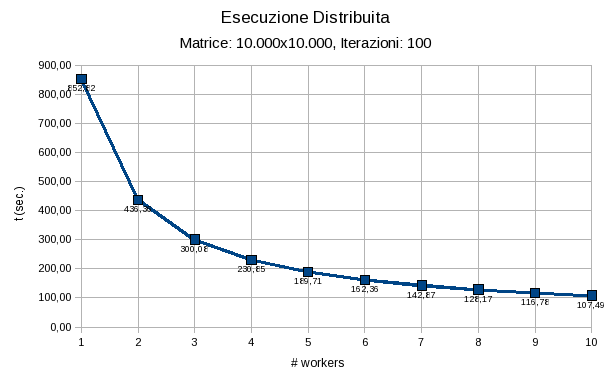
\includegraphics[width=\columnwidth]{grafico-2.png}
  \caption{\emph{Esecuzione distribuita: primo test (matrice grande, poche iterazioni).}}
  \label{fig:graph_2}
\end{figure}
\begin{figure}[ht]
  \centering
  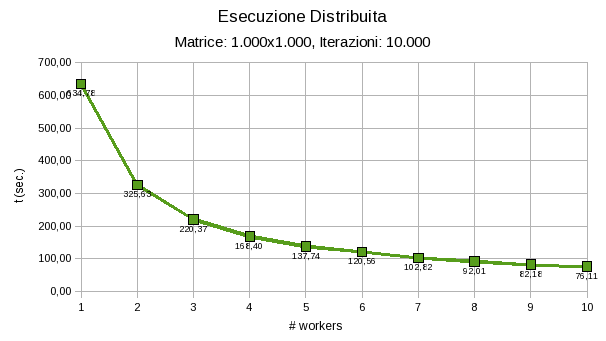
\includegraphics[width=\columnwidth]{grafico-3.png}
  \caption{\emph{Esecuzione distribuita: secondo test (matrice piccola, molte iterazioni).}}
  \label{fig:graph_3}
\end{figure}
I test effettuati sono due: con una matrice di grandi dimensioni (10.000x 10.000) e poche iterazioni (100), di cui l'andamento all'aumentare delle macchine coinvolte \`e rappresentato in figura \ref{fig:graph_2}, e con una matrice di piccole dimensioni (1.000x1.000) ma con tante iterazioni da eseguire (10.000), con l'andamento raffigurato nel grafico in figura \ref{fig:graph_3}. Lo scopo della prova chiaramente \`e verificare un miglioramento dei tempi di esecuzione aumentando il numero di workers coinvolti. Dal grafico del primo test si vede come inizialmente, passando da 1 worker a 2 workers, si hanno netti miglioramenti nel tempo di esecuzione totale, ma questi miglioramenti sono sempre minori aumentando il numero di workers. Questo andamento \`e del tutto normale, infatti passare da un solo worker che deve lavorare sull'intera matrice, a due workers che invece devono eseguire la met\`a dei conti, comporta ovviamente quasi un dimezzamento dei tempi di calcolo; se invece si passa da nove workers a dieci, ogni workers avr\`a comunque meno lavoro da fare, ma con un calo meno significativo rispetto al dimezzamento del passaggio da uno a due. Se ad esempio prendiamo una matrice da 100 colonne, passando da un worker a due, si passa da un PE che lavorava su 100 colonne a due che lavorano su 50 (il carico dimezza), ma se passiamo da nove workers a dieci, si passa da nove PE che avevano circa 11 colonne a dieci che ne hanno 10, percui il carico di lavoro ha un calo minimo. Inoltre si deve considerare che pi\`u workers significa anche pi\`u operazioni di sincronizzazione ad ogni iterazione, percui aumentando i workers si ha un piccolo rallentamento che si deve sottrarre all'aumento di prestazioni dovuto alla distribuzione del carico di lavoro.

Il secondo grafico segue un andamento del tutto analogo al primo, questo mostra il fatto che le operazioni di sincronizzazione, che in questa prova sono 10.000 per ogni coppia di workers, sono veloci e non portano ad un visibile rallentamento del calcolo parallelo.

Da notare che in entrambi i grafici sono riportati solamente i tempi effettivi di esecuzione e non i tempi di utilizzo della cpu, questo perch\'e i due tempi, in entrambe le prove, sono stati sempre praticamente uguali. Bisogna infatti considerare che in questi casi si ha una macchina dedicata per ogni workers, che dedica il suo processore solamente al calcolo della nostra applicazione. Percui, nel caso di sistemi distribuiti su pi\`u macchine, si riescono ad ottenere miglioramenti reali ed effettivi aumentando il numero di workers impiegati. Da fare per\`o particolare attenzione al fatto che se una macchina \`e pi\`u lenta rispetto alle altre, oppure ha altro lavoro da eseguire e non riesce a dedicare a pieno il tempo di utilizzo della cpu all'applicazione, tale macchina porterebbe ad un rallentamento dell'intero processo, dovuto al fatto che \`e necessaria la fase di sincronizzazione al termine di ogni iterazione.

\subsection{Esecuzione a pi\`u processi su una macchina}
In questa prova viene eseguita l'applicazione in una singola macchina, mantenendo invariate le dimensioni della matrice e le iterazioni da eseguire, ed aumentando il numero di workers coinvolti nella computazione con l'obiettivo di diminuire il tempo totale di esecuzione.
\begin{figure}[th]
  \centering
  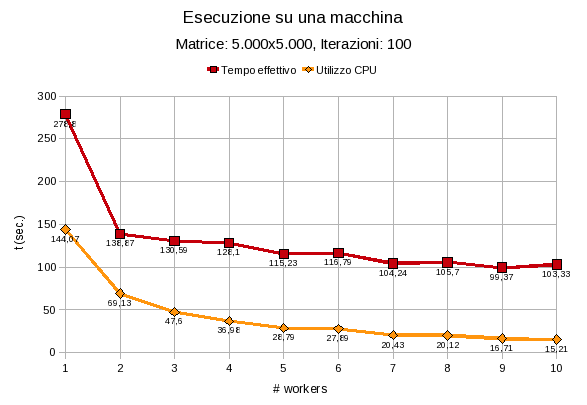
\includegraphics[width=\columnwidth]{grafico-1.png}
  \caption{\emph{Esecuzione dell'applicazione su una singola macchina.}}
  \label{fig:graph_1}
\end{figure}
Ogni workers (oltre allo stage iniziale e finale) sar\`a quindi un processo parallelo e concorrente rispetto agli altri, eseguito su un solo processore della macchina. Il computer utilizzato ha le seguenti caratteristiche:
\begin{itemize}
  \item CPU: Intel Core 2 Duo CPU 2.80GHz
  \item Memoria: 2 GB
\end{itemize}

Nel grafico in figura \ref{fig:graph_1} sono riportati i tempi effettivi e i tempi di utilizzo della cpu all'aumentare del numero di workers impiegati. Si nota subito che i tempi di utilizzo della cpu sono pi\`u bassi e seguono un andamento pi\`u lineare, mentre il tempo effettivo di esecuzione ha un brusco calo passando da uno a due workers, ma poi diminusce in modo minimo all'aumentare del numero di workers. Questo andamento \`e dovuto al fatto che i processi vengono eseguiti su un singolo processore dual core, percui due processi possono essere effettivamente eseguiti in modo parallelo su i due core del processore, e da qui il miglioramento passando da 1 a 2 workers, ma il parallelismo diventa ``virtuale'' per pi\`u di 2 processi, che verrano fatti eseguire a turno sul processore con la politica di scheduling del sistema operativo. Mentre invece il tempo di utilizzo della cpu segue un andamento del tutto analogo a quello su pi\`u macchine distribuite, poich\'e in tal caso viene misurato il lavoro compiuto da ogni processo e non il tempo reale impiegato. Percui, seppur l'impiego di cpu diminuisce aumentando il numero di processi, su una singola macchina si possono ottenere miglioramenti effettivi dalla parallelizzazione solamente utilizzando tanti workers quanti sono i core (o i processori) della macchina stessa, altrimenti il tempo totale dell'esecuzione non diminuisce, ma anzi, pu\`o addirittura aumentare a causa dei tempi persi nella sincronizzazione o per piccoli effetti di starvation dovuti ad uno scheduling non adatto del sistema operativo.
